\documentclass[a4paper,10pt]{article}

\usepackage{graphicx}
\usepackage[ansinew]{inputenc}
\usepackage[spanish]{babel}
\usepackage{listings} 
\usepackage{tabto}
\usepackage{float}
\usepackage[justification=centering]{caption}
\usepackage[T1]{fontenc}
\usepackage{hyperref}
\usepackage{mips}
\usepackage[section]{placeins}
\usepackage{pdfpages}
\usepackage{enumitem}
\usepackage{microtype}
\DisableLigatures[-]{}


\renewcommand{\labelitemi}{$\bullet$}
\renewcommand{\labelitemii}{$\circ$}


\title{		\textbf{Trabajo pr�ctico \#2: datapath}}

\author{	Santiago Fernandez, \textit{Padr�n Nro. 94.489}                     \\
            \texttt{ fernandezsantid@gmail.com }                                              \\[2.5ex]
            Pablo Rodrigo Ciruzzi, \textit{Padr�n Nro. 95.748}                     \\
            \texttt{ p.ciruzzi@hotmail.com }                                              \\[2.5ex]
            Horacio Martinez, \textit{Padr�n Nro. 94.926 }                     \\
            \texttt{ hmk142@hotmail.com }                                              \\[2.5ex]
            \normalsize{2do. Cuatrimestre de 2015}                                      \\
            \normalsize{66.20 Organizaci�n de Computadoras  $-$ Pr�ctica Jueves}  \\
            \normalsize{Facultad de Ingenier�a, Universidad de Buenos Aires}            \\
            \\
            \\
       }
\date{ 26 de Noviembre, 2015}

\begin{document}
\sloppy

\maketitle
\thispagestyle{empty}   % quita el n�mero en la primer p�gina


\begin{abstract}
En este trabajo pr�ctico se ver�n modificaciones a distintos datapaths de una arquitectura MIPS, con el fin de agregar algunas instrucciones que no han sido implementadas en el mismo, y as� poder familiarizarse con dicho concepto. La herramienta utilizada fue el DrMIPS version 2.0 [1][2].
\end{abstract}
\pagebreak 

\tableofcontents
\pagebreak

\section{Introducci�n}
\par DrMIPS nos permite modificar el datapath de la arquietectura MIPS32 y el conjunto de instrucciones. Lo usaremos para agregar las siguientes instrucciones, tres de ellas, \emph{sll}, \emph{srl}, \emph{jr} al datapath monociclo y las otras dos, \emph{j} y \emph{blt} al datapath pipeline.
\par Para lograrlo, agregaremos nuevos componentes al datapath y modificaremos el set de instrucciones, seg�n sea necesario.
\section{Desarrollo}

\subsection{Punto 1}
\par En este �tem, se agregaron las instrucciones \emph{sll} y \emph{srl} al datapath monociclo. Para ello, no fue necesario modificar el datapath, simplemente bast� con agregar las instrucciones al set de instrucciones.
\subsubsection{Set de instrucciones modificado}
Se agregaron las siguientes lineas al campo \emph{instructions} del set:
\begin{verbatim}
"sll": {
        "type": "R", "args": ["reg", "reg", "reg"],
        "fields": {"op": 0, "rs": "#2", "rt": "#3", 
                   "rd": "#1", "shamt": "#3", "func": 0}, 
        "desc": "$t1 = $t2 << $t3 = $t2 * 2^$t3"
},
"srl": {
        "type": "R", "args": ["reg", "reg", "reg"], 
        "fields": {"op": 0, "rs": "#2", "rt": "#3", 
                   "rd": "#1", "shamt": "#3", "func": 2}, 
        "desc": "$t1 = $t2 >> $t3 = $t2 / 2^$t3"
},
\end{verbatim}
\par Lo que esto hace, es definir dos instrucciones nuevas del tipo R, que reciben como argumento tres registros. Luego, el campo \emph{func}, junto con el \emph{aluop}, ser� el que referencie a estras instrucciones en la secci�n de control de la ALU, por lo tanto, al ejecutarlas, la entrada de la ALU ser� la especificada. Por �ltimo, debemos asociar esta entrada con la operaci�n a realizarse, esto lo hacemos en la configuraci�n de la ALU de la siguiente manera:
\begin{verbatim}
"alu": {
        ...
        "control": [
            ...
            {"aluop": 2, "func": 0, "out": {"Operation": 8}},
            {"aluop": 2, "func": 2, "out": {"Operation": 9}},
            ...
        ],
        "operations": {
            ...
            "8": "sll",
            "9": "srl",
            ...
        }
}
\end{verbatim}
\par Esto le indica a la secci�n de control de la ALU, que ante el \emph{aluop}=2 y \emph{func}=0, debe ejecutar la operaci�n 8, en este caso definida como \emph{sll}, an�logamente ocurre con \emph{srl}.
\subsubsection{Pruebas de sll y srl}
\bigskip
\noindent \textbf{Prueba 1:}
\lstset{
	language=[mips]Assembler,
	tabsize=4
}
\lstinputlisting{../punto1/prueba.asm}
\medskip
\textbf{Prueba 2:}
\lstset{
	language=[mips]Assembler,
	tabsize=4
}
\lstinputlisting{../punto1/prueba2.asm}
\medskip
\textbf{Prueba 3:}
\lstset{
	language=[mips]Assembler,
	tabsize=4
}
\lstinputlisting{../punto1/prueba3.asm}
\medskip
\textbf{Prueba 4:}
\lstset{
	language=[mips]Assembler,
	tabsize=4
}
\lstinputlisting{../punto1/prueba4.asm}
\medskip
\textbf{Prueba 5:}
\lstset{
	language=[mips]Assembler,
	tabsize=4
}
\lstinputlisting{../punto1/prueba5.asm}

\subsection{Punto 2}
\subsection{Punto 3}
\subsection{Punto 4}

\section{Conclusiones}

\par Realizar este trabajo pr�ctico nos permiti� familiarizarnos con la arquitectura de CPU MIPS y con el simulador DrMiIPS. Nos sirvi� para comprender como funciona el datapath monociclo y el pipeline, tambi�n para darnos cuenta que hay distintas formas de implementar una instrucci�n. 
\par En algunos casos es posible agregar instrucciones sin modificar el datapath, como en el caso de las instrucciones \emph{sll} y \emph{srl}, pero generalmente requiere el agregado de nuevos componentes, lo que implica m�s costos, un aumento en la complejidad del datapath y posiblemente una disminuci�n en la velocidad de ejecuci�n. Por lo cual, a la hora de elegir si agregar una nueva instrucci�n, deben considerarse estas desventajas.
\par Por �ltimo, pudimos observar que en determinados casos, como en el de \emph{blt}, no es posible agregar una nueva instrucci�n al datapath, sino que es necesario implementarla como una combinaci�n de instrucciones ya existentes.

\newpage

\section{Referencias}
\noindent[1] DrMIPS, \url{https://bitbucket.org/brunonova/drmips/wiki/Home}.\\ \relax
[2] DrMIPS, \url{https://https://github.com/brunonova/drmips}.\\ \relax

\newpage

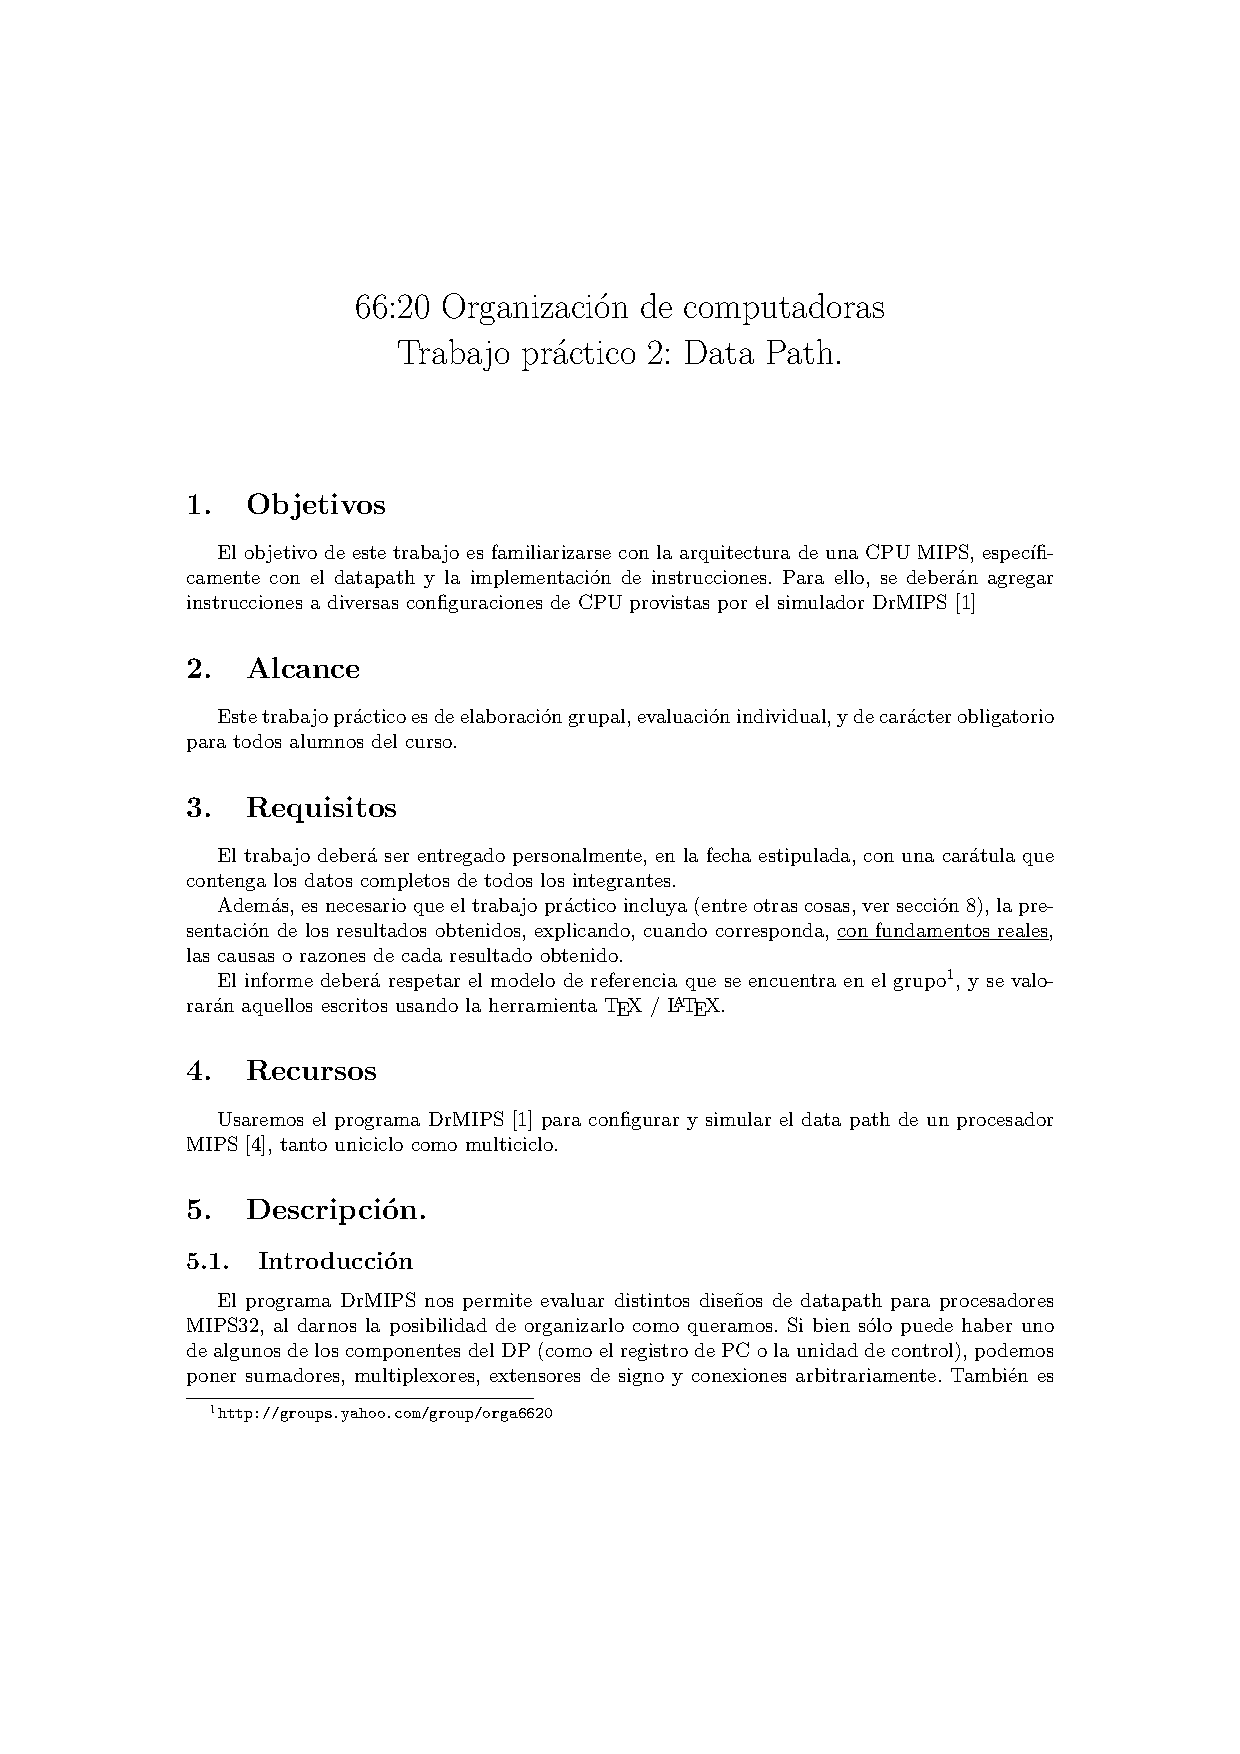
\includepdf[pages={1-3}]{tp2-q2-2015.pdf}

\end{document}